\chapter{Modern Biological Data Management and Analysis}\label{biodata}
From the discovery of the \gls{dna} structure by Watson and Crick in
1953\cite{watson1953molecular} to the sequencing of the human genome in 2001
\cite{venter2001sequence,international2001initial} and the massively parallel
sequencing platforms in the later years\cite{metzker2010sequencing}, the
scientific advances have been tremendous. Today, single week-long sequencing
runs can produce as much data as did entire genome centers just years
ago.\cite{kahn2011future}  These technologies allow researchers to produce data
faster, cheaper and more efficiently, now making it possible to sequence the
entire genome from a patient in less than a days work. In addition to faster
data generation, the new datasets are also higher quality.

Ensuring reproducibility through sharing of analysis code and datasets is
necessary to advance science.\cite{baker2016scientists} From the many obstacles
to replicate results from the most influential papers in cancer
research\cite{reprod}, it is apparent that it is important to thoroughly
document the entire workflow from data collection to interpretable results.
This requires implementing best practices for data storage and processing. Such
best practices are also necessary for large and complex projects where data
collection, analysis, and interpretation may span decades, and therefore done
in several iterations. 

In this chapter we describe our efforts to establish an approach for
reproducible analysis of biological data in a complex epidemiological study. We
first give a short introduction to high-throughput datasets, before describing
the \gls{nowac} study we use as a motivating example. We describe the previous
traditions for data management and analysis, and propose a new approach to
achieve reproducible analyses. Continuing, we show that our approach to manage
research data and code can be used to develop a standardized data analysis
pipeline. Further we provide best practices for data analysis and management. 

% We propose an approach which we have used in the \gls{nowac} study for
% maintaining and analyzing complex systems epidemiology datasets. The approach
% ensures reproducibility, and we believe that it is well adapted for molecular
% data analysis. It enables us to achieve reproducible research through the four
% steps described above. First, we use R since it provides us with an open-source
% programming environment with a range of statistical packages.  Second, we have
% developed an R package with both analysis code, and the datasets from the
% \gls{nowac} study. We document all datasets thoroughly and use version control
% to track both datasets and code over time. Third, we have developed a web
% application, Pippeline, to perform the standardized preprocessing steps for gene
% expression datasets. Fourth, we have developed our own best practices that
% involves reporting results and sharing analyses through reproducible analysis
% reports. 

\section{High-Throughput Datasets for Research and Clinical Use} 
% Cells are the smallest units an organism can be divided into, that still
% possesses the functions performed by living organisms. Within cells we find
% proteins, the working units, found in a wide range of processes.  All cells
% within an organism contain the same genetic information, this genetic
% information is stored within nucleic acids which are responsible for storage,
% transmission and expression. There are two types of nucleic acids, \gls{dna}
% and \gls{rna}.  DNA is responsible for the storage of genetic information,
% while RNA is used in decoding the information stored within DNA. Genes are
% sequences of \gls{dna}, and the human genome consists of approximately 20 500
% genes. These genes specify how proteins are synthesized. In short, DNA is
% transcribed into RNA which are translated to proteins. This is called the
% central dogma of molecular biology. 

It is important to have an understanding the different high-throughput
technologies that are now widely used to study complex diseases such as cancer. 
\gls{dna} sequencing is the process of determining the order of nucleotides
within a strand of \gls{dna}. \gls{hts}, or \gls{ngs}, is a term used to
described newer technology that enables massively-parallel sequencing of
\gls{dna}. \gls{hts} instruments sequence millions of short base pairs, and
we assemble these in the data analysis process. Typical sequencing datasets are
in the size of hundreds of \glspl{gb} per sample. 

While \gls{hts} can study the sequence of bases, microarrays have been used to
study the transcriptome, or the genes actively expressed. While the genome is
mostly fixed for an organism, the transcriptome is continuously changing. These
instruments report the expression levels of many target genes, and
by profiling these we can study which genes are active in the biological sample.
Microarray datasets are in the size of megabytes per sample. 

Another technique to study the transcriptome is to use \gls{rna}-seq technology
based on \gls{hts}. \gls{rna}-seq instruments also read millions of short base
pairs in parallel, and can be used in gene expression analysis. Because of its
higher quality output, \gls{rna}-seq is the successor to microarray technology.
These datasets are also in the size of hundreds of \glspl{gb}.

Precision medicine uses patient-specific molecular information to diagnose and
categorize disease to tailor treatment to improve health
outcome.\cite{national2011toward} Important research goal in precision medicine
are to learn about the variability of the molecular characteristics of
individual tumors, their relationship to outcome, and to improve diagnosis and
therapy.\cite{tannock2016limits} International cancer institutions are therefore
offering dedicated personalized medicine programs, but while the data collection
and analysis technology is emerging, there are still unsolved problems to enable
reproducible analyses in clinical settings. For cancer, \gls{hts}
is the main technology to facilitate personalized diagnosis and
treatment since it enables collecting high quality genomic data from patients
at a low cost. 

\section{Norwegian Women and Cancer (\gls{nowac})}
In this thesis we have used data from the \gls{nowac} study extensively. 
The \gls{nowac} study is a prospective population-based cohort that tracks 34\%
(170.000) of all Norwegian women born between 1943–57.\cite{nowac} The data
collection started in \gls{nowac} in 1991 with surveys to cover, among others,
the use of oral contraceptives and hormonal replacement therapy, reproductive
history, smoking, physical activity, breast cancer, and breast cancer in the
family. The datasets are also integrated with data from The Norwegian Cancer
Registry, and The Cause of Death Registry in Statistics Norway. In addition
to the questionnaire data, the study includes blood samples from 50.000 women,
as well as more than 300 biopsies. From the biological samples the first gene
expression dataset was generated in 2009, and the study now also feature miRNA,
methylation, metabolomics, and \gls{rna}-seq datasets. 

The data in the \gls{nowac} cohort allows for a number of different study
designs. While it is a prospective cohort study, we can also draw a case-control
study from the cohort, or a cross-section of the cohort. From the
\gls{nowac} cohort there has been published a number of research papers that
investigate the questionnaire data. We have also used the gene expression
datasets to explore gene expression signals in blood and interactions between
the tumor and the blood systemic response of breast cancer
patients.\cite{holden2017local, dumeaux2017interactions}. Some analyses
have resulted in patents\cite{blobrec} and commercialization efforts.  While
many interesting patterns and results have been studied, there are still many
unexplored areas in the available datasets.

In the \gls{nowac} study we are a traditional group of researchers, PhD and
Post-Doc students, and administrative and technical staff. Researchers have
backgrounds from statistics, medicine, or epidemiology, and now also computer
science. The administrative and technical staff is responsible for managing the
data, both data collection and data delivery to researchers. 

\subsection{Data Management and Analysis} 
Surveys are the traditional data collection method in epidemiology. But
today, questionnaire responses are increasingly integrated with molecular data.
However, surveys are still important for designing a study that can answer
particular research questions.  In this section we describe how such integrated
data analysis was done in \gls{nowac} before we developed our approach. We
believe many studies have, or are still, analyzing epidemiological data using
previous approach. 

In the \gls{nowac} study we have stored the raw survey and registry data in an
in-house database backed up to an independent storage node. Previously,
researchers had to apply to get data exported from the database by an engineer.
This was typically done through SAS scripts that did some preprocessing, e.g.
selecting applicable variables or samples, before the data was shared to
researchers as SAS data files. The downstream analysis was typically done in
SAS. Researchers used e-mail to communicate and share data analysis scripts, so
there was not a central hub with all the scripts and data. 

In addition to the questionnaire data, the \gls{nowac} study also integrates
with registries which are updated regularly. The datasets from the different
registries are typically delivered as \gls{csv} files to our technical staff,
which are then processed into a standardized format. Since the \gls{nowac} study
is a prospective cohort, a percentage of the women are expected to get cancer
and move from the list of controls into the list of cases. 

In the \gls{nowac} study we have used processed and analyzed outside our
research institution.  The received raw datasets were then stored on a
local server and made available to researchers on demand. Because of the
complexity of the biological datasets, many of these require extensive
pre-processing before they are analysis-ready. 


\section{Enabling Reproducible Research} 
To enable reproducible research in the \gls{nowac} study we have developed a
system for managing and documenting the available datasets, a standardized data
preprocessing and preparation system, and a set of best practices for data
analysis and management. We designed our management and analysis system as a
\gls{sme} that we could later use in the Pippeline system. 

Through nearly a decade of experiences from transcriptomics data analysis, we
identified a set of issues that prevented us from fully ensuring reproducible
data analysis: 
\begin{enumerate} 
    \item 
        It was very difficult and time-consuming to get an overview of previous
        work, and track and understand changes in the analysis process. This was
        because there was no version control of the analysis scripts or
        datasets, and information was passed between researchers using e-mails.
        Also, when members left the group they brought the analysis code with
        them. 
    
    \item It was difficult to keep track of the available datasets, and to
        determine how these had been processed. We had no standard data storage
        platform or structure, and there are limited reports for exported
        datasets given to different research projects.

    \item It was is difficult for new group members to understand both the
        datasets and underlying epidemiological study designs. This was because
        we did not have any centralized location for documenting the datasets.
    
    \item It became difficult to reproduce the results reported in our published
        research manuscripts. This was because we did not have any standard for
        reporting results using reproducible reports. 

    \item There was no standard approach to preprocess and initiate data
        analysis. This was because the different datasets were analyzed by
        different researchers, and there was little tradition for sharing
        reusable code between projects. 
        
\end{enumerate} 

To solve these issues and enable reproducible research in the \gls{nowac} study,
we had to develop a system for managing the data, code, and best practices for
analyzing the data. We started with identifying a set of requirements for a
system to manage and document the different datasets: 

\begin{itemize} 
    \item It should provide users with a single interface to access the
        datasets, their respective documentation, and utility functions to
        access and analyze the data.
    \item It should provide version history for the data and analysis code. 
    \item The system should provide reproducible data analysis
        reports\footnote{Such as an R Markdown file which, when executed,
        generates the output data and optional documentation including plots,
        tables etc.} for any dataset that has been modified in any way. 
    \item It should be portable and reusable by other systems or applications. 
\end{itemize} 

To satisfy the above requirements we developed the \texttt{nowac} R package, a
software package in the R programming language that provides access to all data,
documentation, and utility functions. Since it is a requirement that it should
be reusable we could then implement a data preparation system, Pippeline, ontop
of this R package. We identified a set of requirements for this data
preprocessing and preparation system as well: 

\begin{itemize} 
    \item The data preprocessing and preparation system should provide users
        with an interactive point-and-click interface to generate anlaysis-ready
        datasets from the \gls{nowac} study. 
    \item It should use the \texttt{nowac} R package to retrieve datasets. 
    \item It should provide users with a list of possible options for filtering,
        normalization, and other options required to preprocess a microarray
        dataset.
    \item It should genererate a reproducible report along with any exported
        dataset.
\end{itemize} 

Finally, we developed a set of best practices for data analysis in our study. In
the rest of the section we detail how we built the \texttt{nowac} package, the
Pippeline, and the best practices for data analysis. 

\subsection{The \texttt{nowac} Package} 
The \texttt{nowac} R package is our solution for storing, documenting, and
providing helper functions to analyze the datasets in the \gls{nowac} study. We
use \texttt{git} to version control the analysis code and datasets, and store
the repository on a self-hosted git server.

An R package is just a collection of R code, and optional data, organized with a
pre-defined directory structure. We follow the standards, and have added both
raw data and clean analysis-ready datasets to the R package. These raw datasets
include raw gene expression files straight from the different instruments, as
well as raw files from different health registries. For the clean data stored in
the R package we also provide a full reproducible data analysis report that
includes all processing steps. Clean datasets include analysis-ready data that
have been preprocessed to remove outliers, and questionnaire responses. In our
study, superusers add datasets and document them, while researchers use the
package to access the documentation and use its data analysis functions.  

The first step in organizing the data management and analysis in the
\gls{nowac} study was to identify the possible programming environments that we
could use to develop our approach. While the majority of the researchers that
have worked on the project have used SAS for their analyses of the questionnaire
data, all researchers working on biological data are using R. Because of the
number of additional software  packages, its open-source implantation, and
growing developer community we have opted to implement our approach for managing
and processing to fit the R programming language. 

The great strength of R comes from its many packages for analyzing, plotting,
and interpreting data. An R package consists of a code, documentation, tests,
and data. Bioconductor\cite{bioconductor} and the \gls{cran}\cite{cran} provide
online hosing for many packages, and users can mix and match these
packages to fit their need. 

As of now we have 13 datasets in \texttt{nowac} package. 7 datasets are related
to breast cancer and one dataset for diabetes, uterus, endometrial and lung
cancer respectively. All non breast cancer datasets were designed as prospective
case-control studies.  Breast cancer have one postdiagnostic and 3
hospital-based cross-sectional control-cases datasets. Also, there are two
questionnaire datasets that could be linked to datasets described above.

We bundle together all datasets in the \texttt{nowac} package. This includes
both questionnaire, registry, and gene expression datasets. Because none of these
are particularly large (no single dataset being more than tens of
\glspl{gb}) we are able to distribute them with our R package. Some
datasets require pre-processing steps such as outlier removal before the
analysts can explore the datasets. For these datasets we store both the
\emph{raw} datasets and the analysis-ready clean datasets. We store the
raw datasets in their original format, while clean datasets are stored as R data
files to simplify importing them in R. In addition to the datasets themselves we
store the R code we used to generate the datasets. For clarity, we decorate the
scripts with specially formatted comments that can be used with
knitr\cite{xie2016dynamic} to generate reproducible data analysis reports. These
highlight the transformation of the data from raw to clean, with information
such as removed samples or data normalization methods. 

The documentation of an R package is written as specially formatted R code,
similar to standard markup languages.  The documentation includes information
such as data collection date, instrument types, the persons involved with data
collection and analysis, pre-processing methods etc.  When users install the
\texttt{nowac} package these comments are used to generate interactive help
pages which they can browse in R, either through a command line or through an
\gls{ide} such as RStudio.
We can also export this documentation to a range of different formats, and
researchers can also view them in the R interface. Figure \ref{rpkgfig} shows
the user interface of RStudio where the user has opened the documentation page
for one of the gene expression dataset. 

We use a single repository for the R package, but have opted to use \texttt{git
submodules} for datasets in the R package.  This allows us to separate the
access to the datasets, and the documentation and analysis code. Everyone with
access to the repository can view the documentation and analysis code, but only
superusers have access to the data.  There are however drawbacks to creating one
large repository for both data and code. Since git stores every version of a
file, these types of repositories may become large if the datasets are changing
a lot over time, and are stored in binary formats, e.g. gene expression
datasets. We have explored different techniques to minimize our repository and
have opted to store all datasets as git
submodules\cite{submodule}. Submodules allow us to keep the main repository size
down while still versioning the data. Other alternatives such as
git-raw\cite{gitraw}, git-annex\cite{gitannex} git-lfs\cite{gitlfs} exist, and
these all provide alternative approaches to storing large binary files in the
repository. We have not found that any of these could satisfy our needs, or suit
our preferred usage.  Everyone with access to the repository can view the
documentation and analysis code, but only superusers have access to the data.

\begin{figure}
  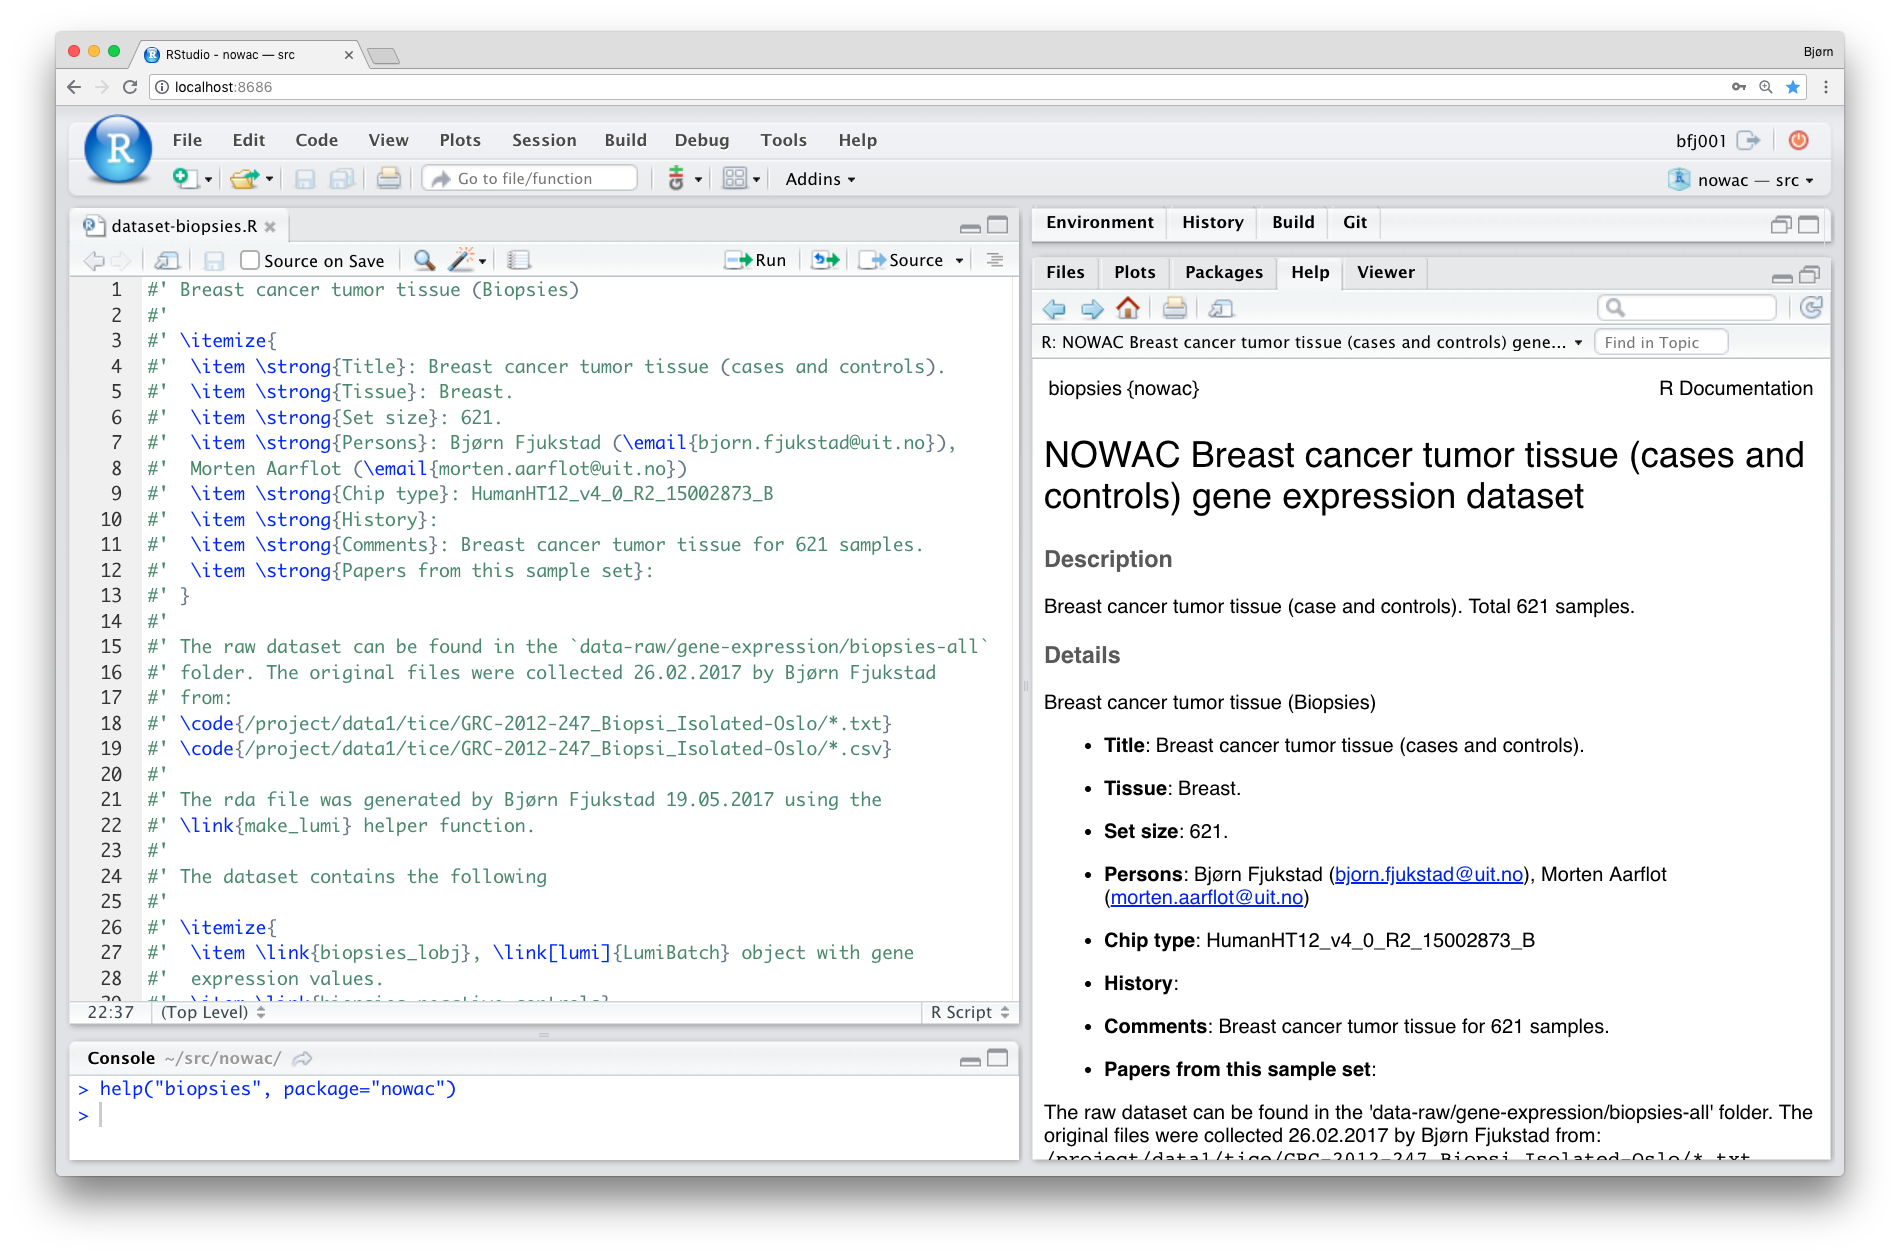
\includegraphics[width=\linewidth]{figures/rpkg.png}
  \caption{A screenshot of the user interface of R Studio viewing the
    documentation help page for the "Biopsies" dataset in the \gls{nowac} study.
    The right-hand panel shows the documentation generated by the code in the
    top left panel. The bottom left panel shows the R command that brought up
    the help page.}
    \label{rpkgfig} 
\end{figure}

\subsection{Processing} 
In the \gls{nowac} package we provide utility functions to get started with the
analysis of our datasets. Because of the specialized nature of the different
research project the \gls{nowac} package only contains helper functions to start
analyzing \gls{nowac} data, e.g. retrieving questionnaire data. 


\section{Standardized Data Analysis}
Analyzing the biological data in the \gls{nowac} study consists of four major
parts as show on Figure \ref{fig:uit_pippeline}.  First, as explained above the
raw datasets are added to the \texttt{nowac} R package and documented thoroughly
by a data manager.  Second, we manually examine the biological datasets to
detect outliers. We add information about outliers to the \texttt{nowac} R
package along with reports that describe why an observation is marked as an
outlier.  Third, the data manager generates an analysis-ready dataset for a
research project using the interactive Pippeline tool. This dataset is
preprocessed, and integrated with questionnaire and registry datasets. Fourth,
researchers analyze the dataset with their tools of choice, but following using
our best practices for data analysis.

\begin{figure}
    \centering
    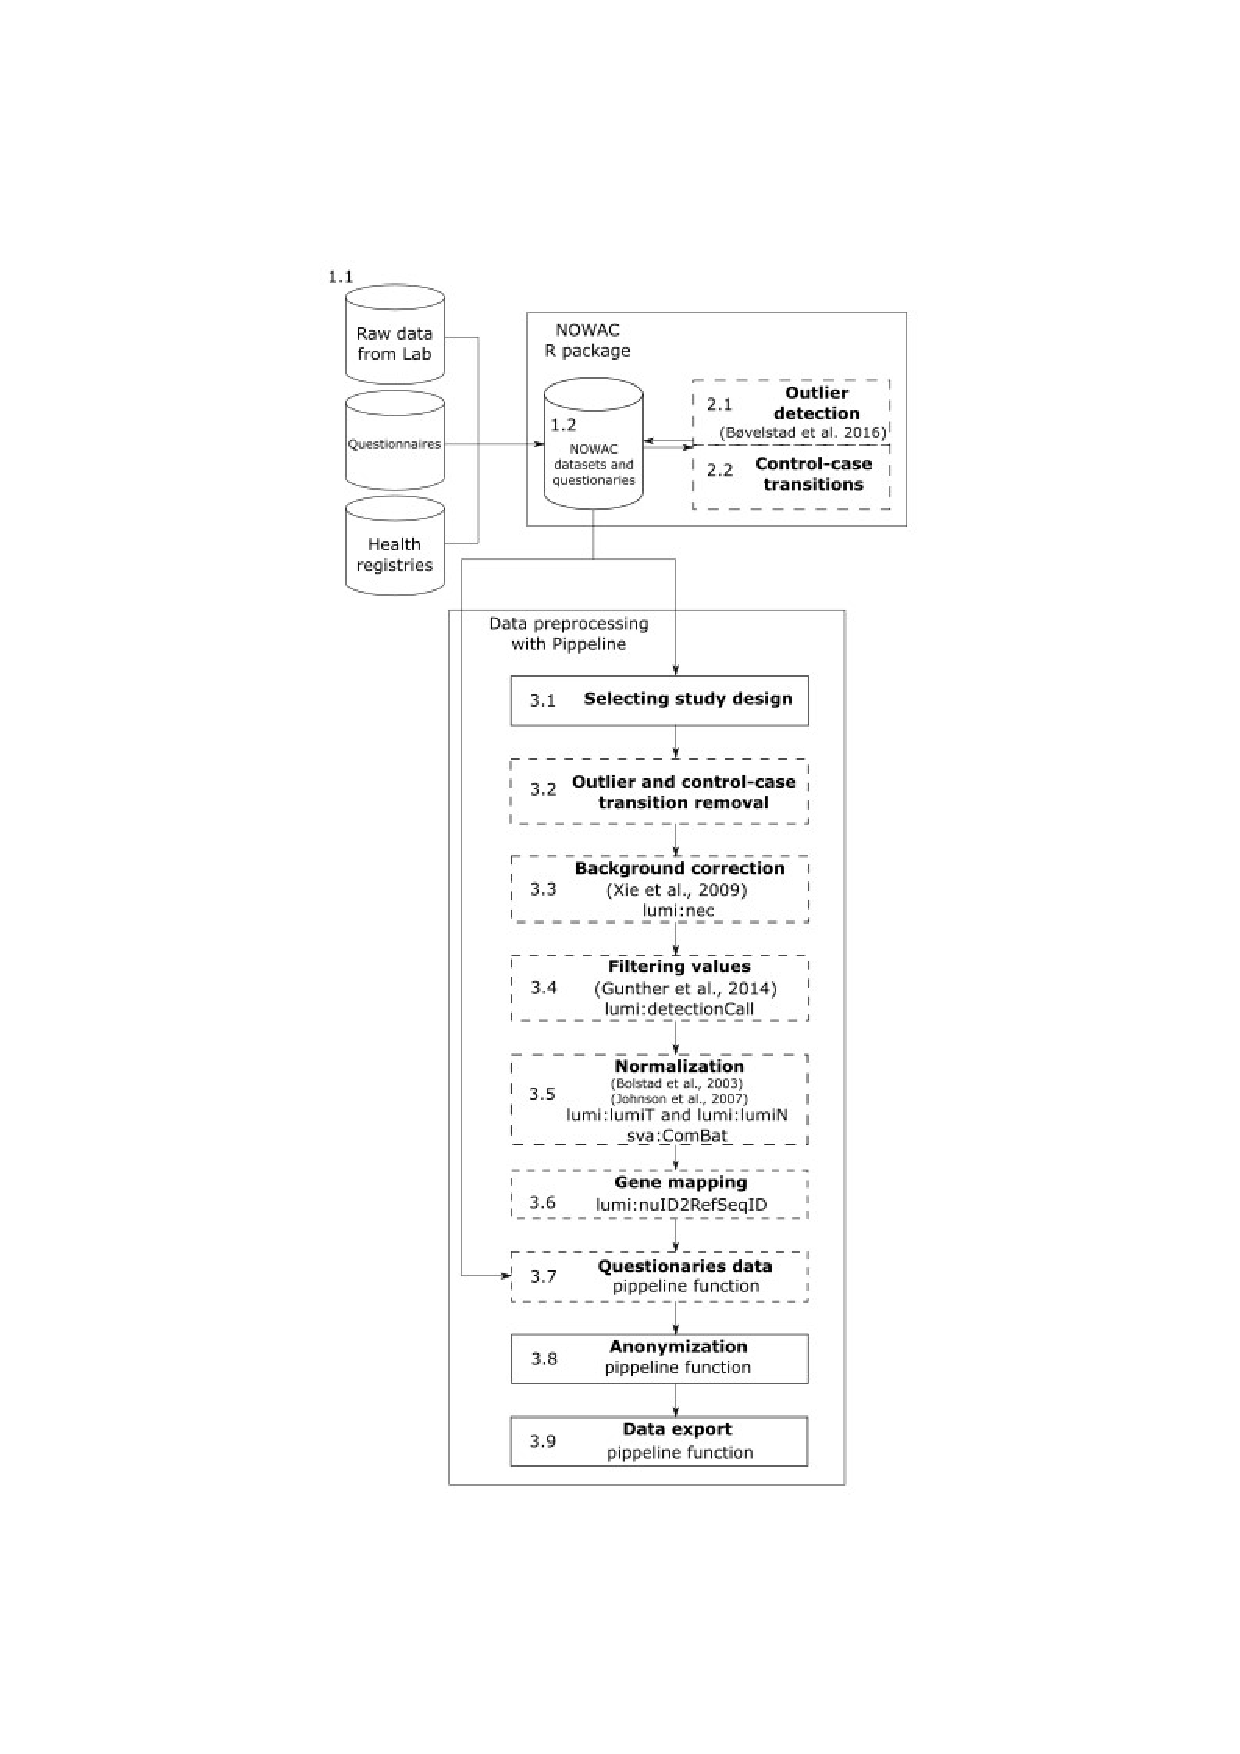
\includegraphics[width=9cm]{figures/uit_pippeline.pdf}
    \caption{The standardized data processing pipeline for gene expression data
    analysis in the \gls{nowac} study. Steps with a dashed line are optional,
    while steps marked with a solid line are mandatory.}
    \label{fig:uit_pippeline}
\end{figure}


\subsection{Pippeline} 
We have developed our preprocessing pipeline for gene expression data as a
point-and-click web application called Pippeline. The web application is
stand-alone and does not require the users to use any command-line tools or have
any programming knowledge. Pippeline generates an analysis-ready dataset by
integrating biological datasets together with questionnaire and registry data,
all found in our \texttt{nowac} package. It uses pre-discovered outliers to
exclude samples, and presents the user with a list of possible processing
options. It exports the analysis-ready R data files together with a reproducible
data analysis report, an R script, that describes all processing steps.  Figure
\ref{fig:scr_filtering} shows the filtering step in Pippeline where users define
at what level they wish to exclude gene expression probes in the dataset. 

The web application is implemented in R using the \texttt{Shiny} framework. It
uses the \texttt{nowac} R package to retrieve all datasets. 

%Users specify details such as what type of study design, e.g. cross-sectional or
%case-control, the data normalization methods, and integration with the
%questionnaires. 

\begin{figure}
    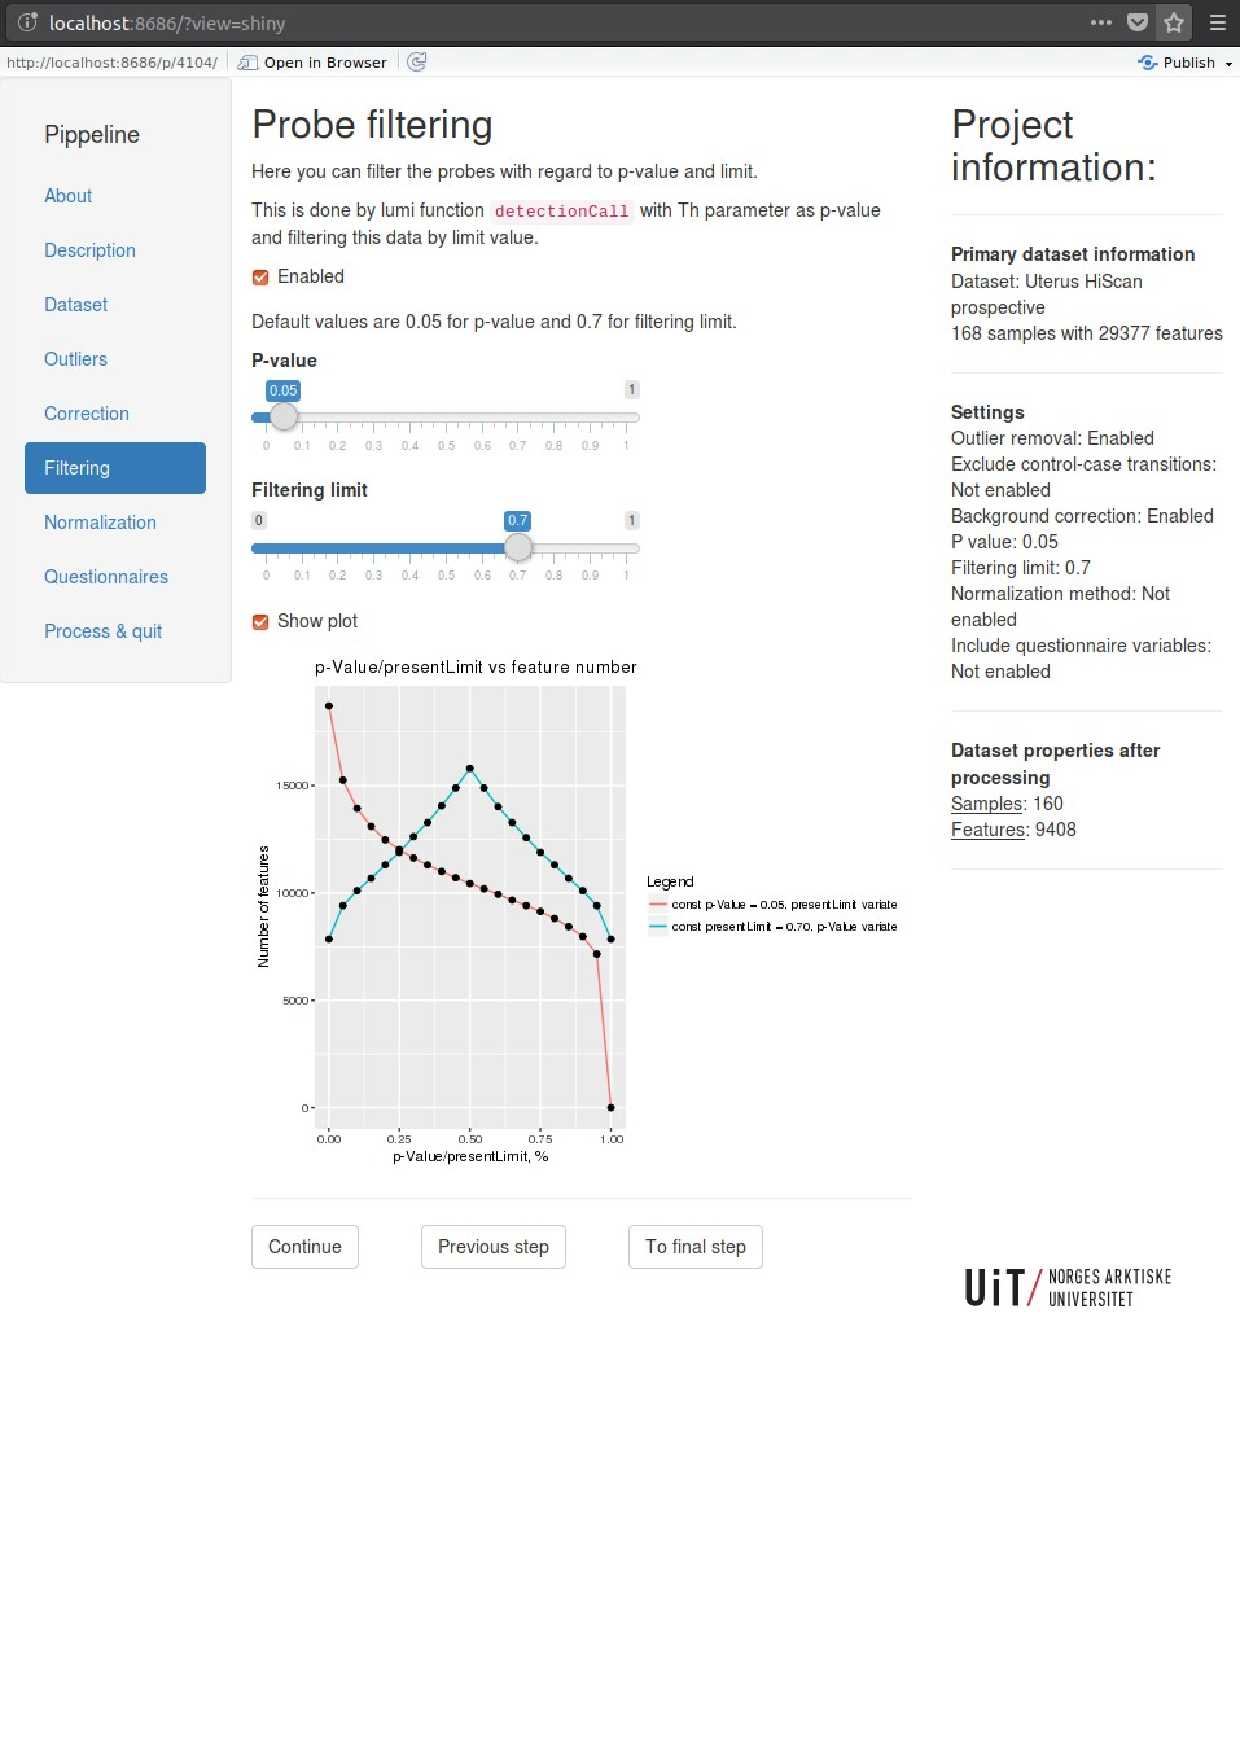
\includegraphics[width=\linewidth]{figures/scr_filtering.pdf}
  \caption{A screenshot of the web-interface of Pippeline. In the screenshot
    users can define at what level they want to filter out probes.}
  \label{fig:scr_filtering}
\end{figure}

\section{Best Practices} 
From our experiences we have developed a set of best practices for researchers
working on data analysis in the \gls{nowac} study. These apply both to
researchers, and developers and the technical staff managing the data in the
study. We believe that we can generalize these to researchers working in
different disciplines. 

\textbf{Document every step in the analysis}. Analysis of modern datasets is a
complex exercise with the possibility of introducing an error in every step.
Analysts often use different tools and systems that require a particular set of
input parameters to produce results. Thoroughly document every step from raw
data to the final tables that go into a manuscript.

In the \gls{nowac} study we write help pages and reports for all datasets, and
the optional pre-processing steps. 

\textbf{Generate reports and papers using code}. With tools such as R
Markdown\cite{rmarkdown} and kntir there are few reasons for decoupling analysis
code with the presentation of the results through reports or scientific papers.
Doing so ensures the correctness reported results from the analyses, and greatly
simplifies reproducing the results in a scientific paper. 

In the \gls{nowac} study we produce reports from R code. These include
pre-processing and data delivery of datasets to researchers. One example of a
report is the analyses done in \cite{kiselev2018transcription} where we
documented the association between PAX6 gene expression and PAX6 target genes.
Through a simple R script we could share the results and underlying analysses.

\textbf{Version control everything}. Both code and data changes over the course
of a research project. Version control everything to make it possible to retrace
changes and the person responsible for them. It is often necessary to roll back
to previous versions or a dataset or analysis code, or to identify the
researches that worked on specific analyses. 

In the \gls{nowac} study we promote the use of git to version control both
source code and data. 

\textbf{Collaborate and share code through \gls{scm} systems}. Traditional
communication through e-mail makes it difficult to keep track of existing
analyses and their design choices both for existing project members and new
researchers. With \gls{scm} hosting systems such as Github developing
analysis code becomes more transparent to other collaborators, and encourages
collaboration. It also simplifies the process or archiving development decisions
such as choosing a normalization method.

In the \gls{nowac} study we collaborate on data analysis through a self-hosted
Gitlab\cite{gitlab} installation. We also open-source our code on
Github. 

\section{Discussion}
There are many approaches to store and analyze biological datasets. Our approach
is targeted towards R users by building an R package, but as we demonstrate in
the next chapters, we have designed systems that interface directly with data
and analyses from outside the R ecosystem. 

One major drawback with the implementation of our approach in the \texttt{nowac}
R package is its size. While microarray datasets are relatively small compared
to sequencing data, when these datasets grow in number the total size grows as
well. This will impact the compile time for the R package, and also its size
when it is shared with other researchers. This is something we hope to address
in future versions. 


\section{Conclusion}
In summary, we believe that there are four rules toward reproducible
analyses:
\begin{itemize} 
    \item Document and version control datasets and analysis code within the
        study. 
    \item Share datasets and analysis code through statistical packages. 
    \item Share and report findings through reproducible data analysis reports. 
    \item Standardize and document common preprocessing and data preparation
        steps.
\end{itemize} 

In this chapter we have demonstrated one approach that we believe help
researchers follow these to enable reproducible research. 


%\subsection{Discussion} 
% large datasets, e.g. sequencing 



% \section{Analysis Pipelines}
% Watchdog:
% https://bmcbioinformatics.biomedcentral.com/articles/10.1186/s12859-018-2107-4
% maybe this one
% http://gopherdata.io/post/more_go_based_workflow_tools_in_bioinformatics/

% \section{Interactive Applications} 
